\subsection{Mean-field approximation revisited}
\label{sec:chap4_mean_field}

We revisit in the following the mean-field approximation by optimising the VR bound, with Bayesian linear regression as an illustrating example. Recall the mean-field approximation factorises over the components of $\mparam = (\theta_1, ..., \theta_D)$: $q(\mparam) = \prod_{i} q_i(\theta_i)$. Re-writing the VR bound (\ref{eq:chap4_vrbound_exact_bound}), we have
\begin{equation*}
\begin{aligned}
\mathcal{L}_{\alpha}(q; \mathcal{D}) &= \frac{1}{1 - \alpha} \log \int \prod_i q_i(\theta_i)  \left( \frac{p(\mparam, \mathcal{D})}{\prod_i q_i(\theta_i)} \right)^{1 - \alpha} d\mparam \\
&= \frac{1}{1 - \alpha} \log \int q_j(\theta_j)^{\alpha} \left( \int \prod_{i \neq j} q_i(\theta_i)  \left( \frac{p(\mparam, \mathcal{D})}{\prod_{i \neq j} q_i(\theta_i)} \right)^{1 - \alpha} d\mparam_{\neq j} \right) d\theta_j \\
&:= \frac{1}{1 - \alpha} \log \int q_j(\theta_j)^{\alpha} \tilde{p}_j(\theta_j)^{1 - \alpha} d\theta_j + \text{const},
\end{aligned}
\end{equation*}
where $\tilde{p}_j(\theta_j)$ denote the ``marginal'' distribution satisfying
\begin{equation*}
\log \tilde{p}_j(\theta_j) = \frac{1}{1 - \alpha} \log \int \prod_{i \neq j} q_i(\theta_i)  \left( \frac{p(\mparam, \mathcal{D})}{\prod_{i \neq j} q_i(\theta_i)} \right)^{1 - \alpha} d\mparam_{\neq j} + \text{const}.
\end{equation*}
Now maximising the VR bound (when $\alpha > 0$, and for $\alpha < 0$ we minimise the bound) is equivalent to minimising $\mathrm{D}_{\alpha}^{R}[q_j||\tilde{p}_j]$ (for $\alpha > 0$, and when $\alpha < 0$ we minimise $\mathrm{D}_{1 - \alpha}^{R}[\tilde{p}_j||q_j]$), which means $\log q_j(\theta_j) = \log \tilde{p}_j(\theta_j) + \text{const}$ is the only global optimum of the mean-field approximation procedure. One can verify that when $\alpha \rightarrow 1$ it recovers the traditional variational mean-field approximation (see Section \ref{sec:chap2_mean_field_vi})
\begin{equation*}
\lim_{\alpha \rightarrow 1} \log \tilde{p}_j(\theta_j) = \int \prod_{i \neq j} q_i(\theta_i) \log p(\mparam, \mathcal{D}) d\mparam_{\neq j} + \text{const},
\end{equation*}
and when $\alpha \rightarrow 0$ the fixed point equation returns the exact marginal of the posterior distribution:\footnote{This is \emph{not} the unique fixed point of $\lim_{\alpha \rightarrow 0} \mathcal{L}_{\alpha} = \mathcal{L}_0$, since $\mathcal{L}_0 = \text{const}$ when $q$ has full support.} 
$$\lim_{\alpha \rightarrow 0} \tilde{p}_j(\theta_j) = p(\theta_j |\mathcal{D}).$$

Now consider Bayesian linear regression with 2-D input $\bm{x}$ and 1-D output $y$, as an example:
\begin{equation*}
\mparam \sim \mathcal{N}(\mparam; \bm{\mu}_0, \bm{\Lambda}_0^{-1}), \quad 
y|\bm{x} \sim \mathcal{N}(y; \mparam^T \bm{x}, \sigma^2).
\end{equation*}
Given the observations $\mathcal{D} = \{\bm{x}_n, y_n \}$, the posterior distribution of $\mparam$ can be computed analytically as $p(\mparam|\mathcal{D}) = \mathcal{N}(\mparam; \bm{\mu}, \bm{\Lambda}^{-1})$ with $\bm{\Lambda} = \bm{\Lambda}_0 + \frac{1}{\sigma^2} \sum_n \bm{x}_n \bm{x}_n^T$ and $\bm{\Lambda} \bm{\mu} = \bm{\Lambda}_0 \bm{\mu}_0 + \frac{1}{\sigma^2} \sum_n y_n \bm{x}_n$. To see how the mean-field approach works we explicitly write down the elements of the posterior parameters
\begin{equation*}
\bm{\mu} = \begin{pmatrix} \mu_1 \\ \mu_2 \end{pmatrix}, \quad
\bm{\Lambda} = \begin{pmatrix} \Lambda_{11} & \Lambda_{12} \\ \Lambda_{21} & \Lambda_{22} \end{pmatrix}, 
\quad \Lambda_{12} = \Lambda_{21},
\end{equation*}
and define $q_i(\theta_i) = \mathcal{N}(\theta_i; m_i, \lambda_i^{-1})$ as a univariate Gaussian distribution. Then
\begin{equation*}
\begin{aligned}
\log q_1 &= \frac{1}{1 - \alpha} \log \int q_2(\theta_2)  \left( \frac{p(\mparam, \mathcal{D})}{q_2(\theta_2)} \right)^{1 - \alpha} d\theta_2 + \text{const} \\
&= \frac{1}{1 - \alpha} \log \int \exp \left[ -\frac{1 - \alpha}{2} (\mparam - \bm{\mu})^T \bm{\Lambda} (\mparam - \bm{\mu}) - \frac{\alpha}{2} \lambda_2 (\theta_2 - m_2)^2 \right] d\theta_2 + \text{const} \\
&= \frac{1}{1 - \alpha} \log \int \mathcal{N}(\mparam; \bm{\mu}, \tilde{\bm{\Sigma}}) d\theta_2 + \text{const} \\
&= \log \mathcal{N}(\theta_1; m_1, \lambda^{-1}) + \text{const}
\end{aligned}
\end{equation*}
where the new mean $m_1$ and the precision $\lambda_1$ satisfies
\begin{equation*}
\begin{aligned}
m_1 = \mu_1 + C_1(\mu_2 - m_2), \quad C_1 = \frac{\alpha \lambda_2 \Lambda_{12}}{(1 - \alpha) |\bm{\Lambda}| + \alpha \lambda_2 \Lambda_{11}}, \\
\lambda_1 = \Lambda_{11} - (1 - \alpha) \Lambda_{12} ((1 - \alpha) \Lambda_{22} + \alpha \lambda_2)^{-1} \Lambda_{21}.
\end{aligned}
\end{equation*}
One can derive the terms $m_2$ and $C_2$ for $q_2$ in the same way, and show that $\bm{m} = \bm{\mu}$ is the only stable fixed point of this iterative update. So we have $q_1 = \mathcal{N}(\theta_1; \mu_1, \lambda_1^{-1})$, and similarly $q_2 = \mathcal{N}(\theta_1; \mu_2, \lambda_2^{-1})$ with $\lambda_2 = \Lambda_{22} - (1 - \alpha) \Lambda_{21} ((1 - \alpha) \Lambda_{11} + \alpha \lambda_1)^{-1} \Lambda_{12}$. In this example $\lambda_1$, $\lambda_2$ are feasible for all $\alpha$, and solving the fixed point equations, finally we have the stable fixed point as
\begin{equation*}
\lambda_1 = \rho_{\alpha} \Lambda_{11}, \quad \lambda_2 = \rho_{\alpha} \Lambda_{22}, \quad 
\rho_{\alpha} = \frac{1}{2 \alpha} \left[ (2\alpha - 1) + \sqrt{1 - \frac{4\alpha (1 - \alpha) \Lambda_{12}^2}{\Lambda_{11} \Lambda_{22}}} \right].
\end{equation*}
The other solution for the quadratic formula is eliminated since it violates the assumptions that $\lambda_1 > 0$ (when $0 < \alpha < 1$) and $|\mathcal{L}_{\alpha}| < +\infty$ (when $\alpha < 0$ or $\alpha > 1$, since it requires $|\alpha \text{diag}(\bm{\lambda}) + (1 - \alpha)\bm{\Lambda}| > 0$). Thus the stable fixed point in this case is unique.

One can show that $\lim_{\alpha \rightarrow 1} \lambda_1 = \Lambda_{11}$ (the precision of the conditional distribution $p(\theta_1 | \theta_2, \data)$), $\lim_{\alpha \rightarrow 0} \lambda_1 = \Lambda_{11} - \Lambda_{12} \Lambda_{22}^{-1} \Lambda_{21}$ (the precision of the marginal distribution $p(\theta_1|\data)$), and $\lim_{\alpha \rightarrow \pm \infty} \lambda_1 = \Lambda_{11} \pm |\Lambda_{12}| \sqrt{\Lambda_{11} \Lambda_{22}^{-1}}$ (similar results for $\lambda_2$). Also $\rho_{\alpha}$ is continuous and non-decreasing in $\alpha$. This means one can interpolate between mass-covering ($\alpha \rightarrow -\infty$) and zero-forcing ($\alpha \rightarrow +\infty$, when using uni-modal approximations it is usually called mode-seeking) behaviour by increasing $\alpha$ values. 

We visualise the analytical results for Bayesian linear regression in Figure \ref{fig:chap4_vrbound_linear_regression_posterior} and  \ref{fig:chap4_vrbound_linear_regression_energy}. First as predicted, increasing $\alpha$ returns more confident estimate. Also notice that $\alpha \rightarrow +\infty$ (in cyan) returns non-zero uncertainty estimates (although it is more over-confident than VI) which is different from the maximum a posteriori (MAP) method that only returns a point estimate. Second, setting $\alpha = 0.0$ (in green) returns $q(\mparam) = \prod_i p(\theta_i|\mathcal{D})$ and the exact marginal likelihood $\log p(\mathcal{D})$ (Figure \ref{fig:chap4_vrbound_linear_regression_energy}). Also the approximate MLE is less biased for $\alpha = 0.5$ (in blue) since now the tightness of the bound is less hyper-parameter dependent.

\begin{figure}[t]
 \centering
 \subfigure[Approximated posterior.]{
 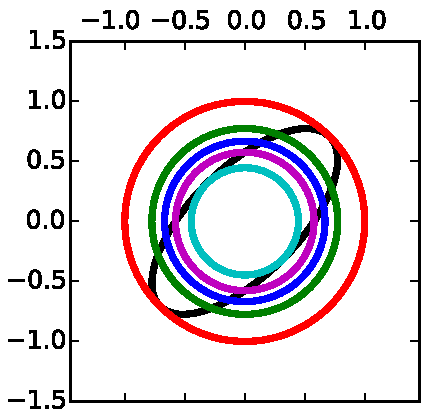
\includegraphics[width=0.24\linewidth]{Chapter4/figs/approx.pdf}
 \label{fig:chap4_vrbound_linear_regression_posterior}}
 \hspace{0.5in}
 \subfigure[Hyper-parameter optimisation.]{
 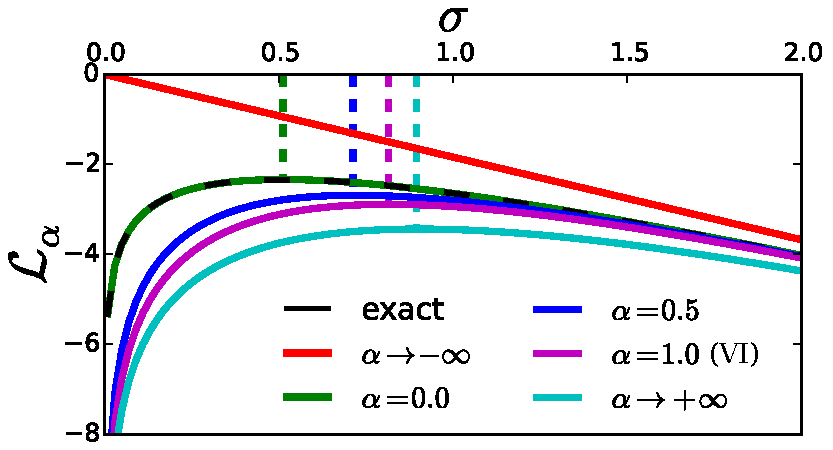
\includegraphics[width=0.45\linewidth]{Chapter4/figs/log_evidence.pdf}
 \label{fig:chap4_vrbound_linear_regression_energy}}
 \caption{Mean-Field approximation for Bayesian linear regression (with one-sigma contours). C.f. Figure \ref{fig:chap2_mean_field}. In this case $\bm{\varphi} = \sigma$ the observation noise variance. As expected when $\alpha = 0$ the resulting bound coincides with the exact log marginal (see the green-black curve). The bound is tight as $\sigma \rightarrow +\infty$, biasing the VI solution to large $\sigma$ values.}
\end{figure}
